\documentclass[10pt,conference,compsocconf]{IEEEtran}

% CS-433 Project 1 report, using the official course paper style.
\usepackage[T1]{fontenc}
\usepackage{microtype}
\usepackage{graphicx}
\usepackage{booktabs}
\usepackage{tabularx}
\usepackage{array}
\usepackage[hidelinks]{hyperref}

\newcolumntype{Y}{>{\raggedright\arraybackslash}X}
\newcommand{\code}[1]{\texttt{#1}}
\renewcommand{\arraystretch}{1.05}

\hypersetup{
  pdftitle={Heart-Disease Classification from BRFSS},
  pdfauthor={Jiawei Lin, Reza Abbasi, Neil Chadli},
  pdfsubject={EPFL CS-433 Machine Learning Project 1}
}

\begin{document}

\title{Heart-Disease Classification from BRFSS}

\author{
  Jiawei Lin \quad Reza Abbasi \quad Neil Chadli\\
  \textit{EPFL, Lausanne, Switzerland}\\
  {\small
  \href{mailto:jiawei.lin@epfl.ch}{jiawei.lin@epfl.ch} \quad
  \href{mailto:reza.abbasi@epfl.ch}{reza.abbasi@epfl.ch} \quad
  \href{mailto:neil.chadli@epfl.ch}{neil.chadli@epfl.ch}}
}

\maketitle

\begin{abstract}
We classify whether a respondent in the 2015 Behavioral Risk Factor
Surveillance System (BRFSS) reports coronary heart disease or myocardial
infarction. Only 8.83\% of the training labels are positive, so we optimize
positive-class F1 instead of accuracy. Our five-fold pipeline combines four
missing-aware gradient-boosted decision tree (GBDT) models with a wide
logistic model and reaches 0.4485 out-of-fold F1. Ablations show that
preserving unanswered survey items and modeling nonlinear interactions
provide the main gains. The model classifies reported disease status; it is
not a predictor of future clinical risk.
\end{abstract}

\section{Introduction}

The course dataset contains 328,135 labeled respondents, 109,379 test
respondents, and 321 BRFSS variables~\cite{cdc2015}. There are 28,975 positive
training examples. An always-negative classifier would therefore obtain
91.17\% accuracy while detecting no positive cases. We use F1, the harmonic
mean of precision and recall, because it rewards a model only when it both
finds positive cases and avoids excessive false alarms.

Our main contribution is to preserve missing answers instead of replacing
them with an average value. BRFSS uses conditional survey paths, so an
unanswered item can reveal which questions a respondent was asked. We test
this choice against course-method baselines, then evaluate whether a nonlinear
model and an ensemble add further improvement. All learning code uses only
NumPy and the Python standard library.

\section{Models and Methods}

\subsection{Data preparation}

We remove 30 administrative and survey-design columns, leaving 291 model
variables. Values meaning ``do not know,'' ``refused,'' or ``not asked'' are
treated as missing; values meaning ``none'' are mapped to zero. Every learned
preprocessing quantity is fitted using training data only.

The two model families receive different representations. For trees, each
variable is mapped to at most 64 observed-value bins plus a missing bin, and
every split learns whether missing values go left or right. For the linear
model, low-cardinality variables are one-hot encoded. Continuous variables
are clipped, standardized, and expanded with ten quantile-bin indicators;
variables that contain missing training values also receive an explicit
missingness flag.

% A full-width figure is placed at the top of the page after its source, so
% it is declared here, on page 1, to appear at the top of page 2.
\begin{figure*}[t]
  \centering
  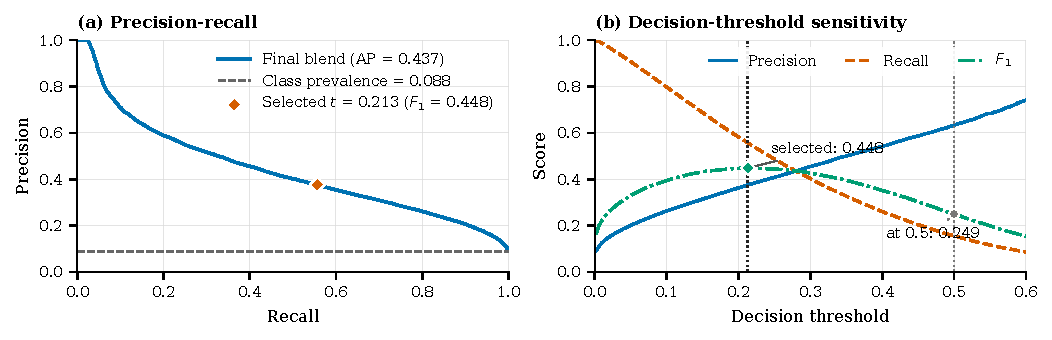
\includegraphics[width=\textwidth]{figures/oof_evaluation_panels.pdf}
  \caption{Out-of-fold evaluation of the final blend ($n=328{,}135$).
  (a) Precision--recall curve; the dashed line is class prevalence and the
  diamond is the selected operating point. (b) Precision, recall, and F1 as
  the decision threshold changes; markers compare the selected and default
  cutoffs.}
  \label{fig:evaluation}
\end{figure*}

\subsection{Predictive models}

We first evaluate ridge regression and regularized logistic regression from
the required course implementations, both with $\lambda=10^{-4}$. They use a
bias column and standardized variables whose missing values are set to the
training mean; the flagged variants add centered missingness indicators.
Logistic regression runs 10,000 gradient steps of size $1/L$, where $L$ is the
Lipschitz constant of the gradient. The wide logistic model then uses the
expanded linear features, Newton optimization, and an $L_2$ penalty of
$10^{-4}$.

The nonlinear component is a NumPy implementation of logistic tree boosting,
following the regularized formulation of Chen and Guestrin~\cite{chen2016}.
Each GBDT has depth 8, learning rate 0.03, minimum leaf size 50,
row/column sampling rates 0.85/0.40, and $L_2=10$. Four models use seeds
1--4 and contain 566, 550, 598, and 583 trees after model selection. Their
mean probability is blended with the wide logistic score:

\begin{equation}
p(x)=0.85\left(\frac{1}{4}\sum_{k=1}^{4}p_{\mathrm{GBDT},k}(x)\right)
     +0.15\,p_{\mathrm{logistic}}(x).
\end{equation}

The final classifier predicts $+1$ when $p(x)\geq0.2131$.

\subsection{Validation protocol}

We use five stratified folds with seed 2026. Within each fold, preprocessing
is fitted on the other four folds and applied to the held-out fold. This
produces one out-of-fold probability per training respondent. We choose the
F1 threshold from the pooled out-of-fold predictions and additionally select
each fold's threshold using only the other four folds' predictions. After
model selection, every component is refitted on all labeled rows.

\section{Results}

Table~\ref{tab:ablation} reports one sequence of changes under the same five
folds. Missingness flags improve ridge F1 by 0.009. Matching the loss to the
binary task and expanding the linear features add 0.012 in total. The largest
later gain comes from nonlinear interactions, while averaging and blending
add a smaller final improvement.

\begin{table}[t]
  \caption{Five-fold ablation. Higher F1 is better; $\Delta$ is relative to
  the preceding row.}
  \label{tab:ablation}
  \centering
  \footnotesize
  \begin{tabularx}{\columnwidth}{@{}Yrr@{}}
    \toprule
    \textbf{System} & \textbf{F1} & \textbf{$\Delta$} \\
    \midrule
    Ridge regression & 0.420 & -- \\
    Ridge + missing flags & 0.429 & +0.009 \\
    Reg. logistic + flags & 0.437 & +0.008 \\
    Wide logistic & 0.441 & +0.004 \\
    Single GBDT (mean over seeds) & 0.447 & +0.006 \\
    Four-GBDT average + logistic blend & \textbf{0.448} & +0.001 \\
    \bottomrule
  \end{tabularx}
\end{table}

Figure~\ref{fig:evaluation} separates ranking performance from threshold
selection. Panel (a) shows the pooled precision--recall trade-off. Panel (b)
shows that the selected threshold 0.2131 balances precision 0.3756 and recall
0.5563 for F1 0.4485, whereas the default 0.5 cutoff gives F1 0.2494.
Selecting each fold's threshold using only the other folds gives F1 0.4477,
just 0.0008 below the pooled result.

Table~\ref{tab:checks} reports the exact ensemble and validation checks.
The threshold-free area under the ROC curve (AUC) and average precision (AP)
improve slightly with averaging and blending, while the cross-fold threshold
result stays close to the pooled score.

\begin{table}[t]
  \caption{Validation and ensemble checks.}
  \label{tab:checks}
  \centering
  \footnotesize
  \begin{tabularx}{\columnwidth}{@{}Yrrr@{}}
    \toprule
    \textbf{System or evaluation} & \textbf{F1} & \textbf{AUC} & \textbf{AP} \\
    \midrule
    Default threshold (0.5) & 0.2494 & -- & -- \\
    Cross-fold threshold selection & 0.4477 & -- & -- \\
    Wide logistic & 0.4406 & 0.8656 & 0.4220 \\
    Best single GBDT & 0.4471 & 0.8703 & 0.4348 \\
    Four-GBDT average & 0.4481 & 0.8707 & 0.4364 \\
    Final blend & \textbf{0.4485} & \textbf{0.8708} & \textbf{0.4368} \\
    \bottomrule
  \end{tabularx}
\end{table}

\section{Discussion}

The experiments support a narrow conclusion: unanswered questions carry
useful signal for classifying reported disease status in this questionnaire.
That strength is also the main limitation. For example, \code{HAREHAB1}, a
rehabilitation question, is observed for only 758 training respondents, all
positive.
Such follow-up questions occur after a cardiovascular event and may partly
reveal the target. The system must therefore not be interpreted as a screening
tool for future risk, and its routing patterns may not transfer to a different
survey.

The validation estimate is not fully independent: GBDT early stopping uses
the fold later scored, and the pooled threshold is selected from the same
out-of-fold predictions. We did not evaluate probability calibration or use a
separate holdout for the final ensemble. The reported scores should therefore
be read as internal model-selection results rather than an external estimate
of clinical performance.

\section{Reproducibility and Conclusion}

The complete source, saved submitted model, prediction file, and exact
commands are in the \href{https://github.com/neilc720/ml-project-1}{public
repository}. The default \code{run.py} entry point loads the model, writes the
submission, and verifies byte identity; its \code{-{}-train} option repeats
cross-validation, threshold selection, and full-data refitting. Separate
evaluation and course-baseline scripts reproduce the reported metrics, and
\code{implementations.py} contains all six required functions.

Preserving survey missingness is the most important contribution: it improves
a course baseline before the model family changes. Missing-aware nonlinear
trees provide the next clear gain, whereas seed averaging and blending offer a
modest refinement. This sequence of controlled comparisons explains both the
final performance and the limits of what the model has learned.

\begin{thebibliography}{1}

\bibitem{cdc2015}
Centers for Disease Control and Prevention, ``2015 BRFSS Survey Data and
Documentation.'' [Online]. Available:
\url{https://www.cdc.gov/brfss/annual_data/annual_2015.html}

\bibitem{chen2016}
T. Chen and C. Guestrin, ``XGBoost: A scalable tree boosting system,'' in
\textit{Proc. 22nd ACM SIGKDD Int. Conf. Knowledge Discovery and Data Mining},
2016, pp. 785--794, doi: 10.1145/2939672.2939785.

\end{thebibliography}

\end{document}
